\begin{table*}[t]
\centering
\resizebox{\textwidth}{!}{
\begin{tabular}{lcccccccc}
\toprule
	\textbf{Model} & \textbf{GSM8K} & \textbf{MATH-500} & \textbf{AIME2024} & \textbf{AIME2025} & \textbf{AMC2023} & \textbf{OlympiadBench} & \textbf{AVG} \\
	\midrule
	Llama-3.1-8B-Instruct    & 75.89 & 35.20 & 4.17 & 1.04 & 23.59 & 12.00 & 25.32 \\
	\texttt{\ \ + 20K Gemini-Distill-Data}   & 54.89 & 22.60 & 1.04 & 0.63 & 12.03 & 7.41 & 16.43  \\
	\texttt{\ \ + 20K Claude4-Distill-Data}  & 63.76 & 35.80 & 1.04 & 0.83 & 23.44 & 13.48 & 23.06   \\
	\midrule
	Qwen-2.5-32B-Base        & 53.68 & 33.40 & 9.17 & 2.29 & 35.63 & 15.85 & 25.00  \\
	\texttt{\ \ + 20K Gemini-Distill-Data}   & 52.54 & 20.20 & 1.88 & 0.63 & 21.41 & 12.44 & 18.18  \\
	\texttt{\ \ + 20K Claude4-Distill-Data}  & 63.31 & 37.80 & 2.92 & 0.83 & 28.91 & 17.78 & 25.26  \\
	\midrule
	Qwen-2.5-32B-Instruct    & 93.71 & 81.00 & 15.60 & 14.17 & 69.84 & 42.22 & 52.76 \\
	\texttt{\ \ + 20K Gemini-Distill-Data}   & 63.68 & 32.80 & 15.00 & 2.92 & 35.63 & 19.11 & 28.19  \\
	\texttt{\ \ + 20K Claude4-Distill-Data}  & 76.88 & 54.80 & 17.71 & 13.96 & 55.00 & 30.96 & 41.55  \\
\bottomrule
\end{tabular}
}
\caption{来自 Gemini 与 Claude 的蒸馏结果。}
\label{tab:distill}
\end{table*}
\begin{table*}[t]
\centering
\resizebox{\textwidth}{!}{
\begin{tabular}{lcccccccc}
\toprule
	\textbf{Model} & \textbf{GSM8K} & \textbf{MATH-500} & \textbf{AIME2024} & \textbf{AIME2025} & \textbf{AMC2023} & \textbf{OlympiadBench} & \textbf{AVG} \\
	\midrule
	Llama-3.1-8B-Instruct    & 75.89 & 35.20 & 4.17 & 1.04 & 23.59 & 12.00 & 25.32 \\
	\texttt{\ \ + 20K OSS-Summarized}   & 54.89 & 22.60 & 1.04 & 0.63 & 12.03 & 7.41 & 16.43  \\
	\texttt{\ \ + 20K QwQ-Summarized}  & 63.76 & 35.80 & 1.04 & 0.83 & 23.44 & 13.48 & 23.06\\
	\midrule
	Qwen-2.5-7B-Instruct & 83.24 & 74.00 & 12.50 & 7.08 & 22.66 & 38.07 & 39.59 \\
    \texttt{\ \ + 20K OSS-Summarized} & 82.34 & 72.60 & 12.50 & 6.46 & 21.41 & 27.70 & 37.17  \\
    \texttt{\ \ + 20K QwQ-Summarized} & 82.71 & 71.80 & 11.88 & 6.25 & 22.97 & 25.04 & 36.77  \\
	\bottomrule
\end{tabular}
}
\caption{将 OpenAI-OSS 与 QwQ 的 Long CoT 轨迹做摘要后的训练结果。}
\label{tab:summarization}
\end{table*}

\begin{figure*}[t]
    \centering
    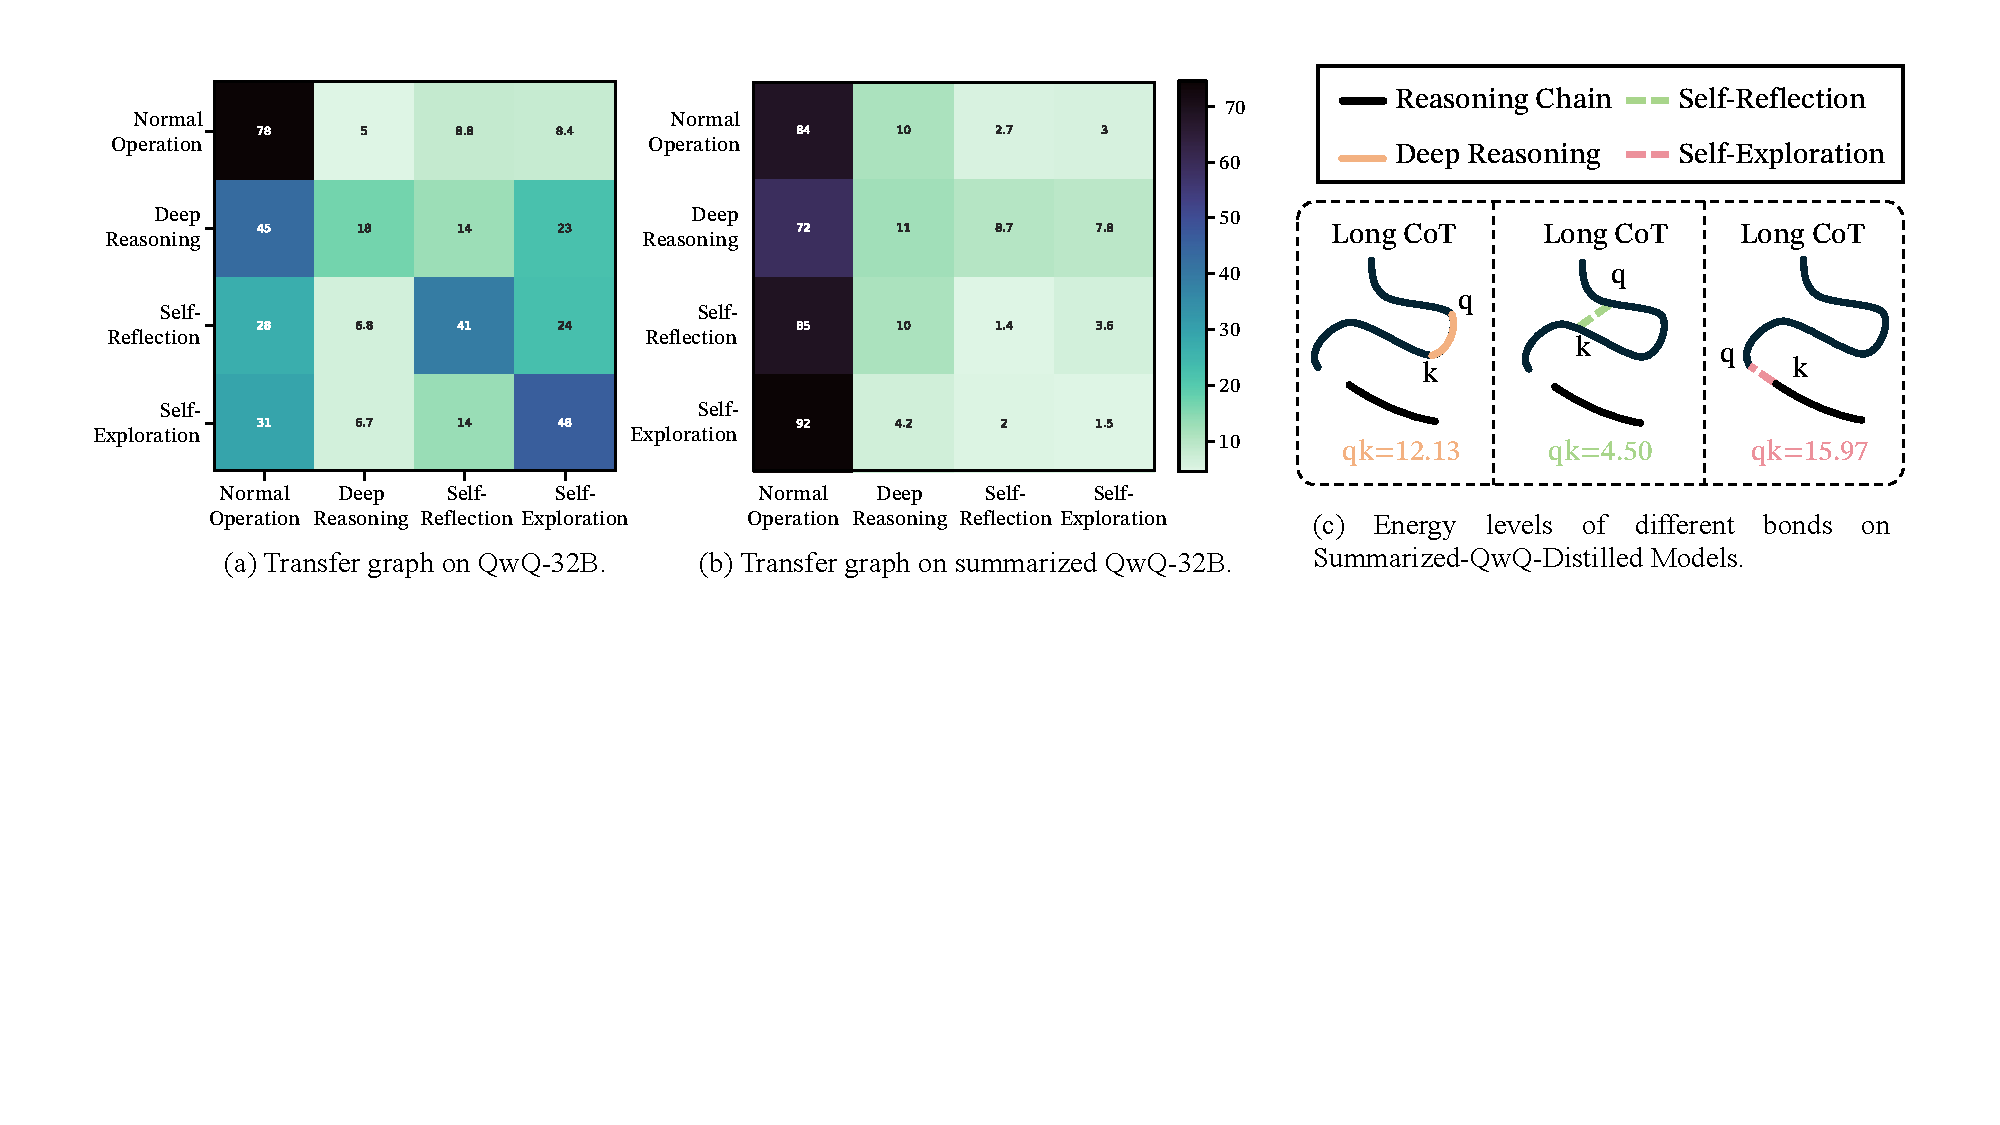
\includegraphics[width=0.98\textwidth]{figures/summary.pdf}
    \caption{QwQ 摘要轨迹的推理行为分布。}
    \label{fig:summary}
\end{figure*}

\section{劣化的分子结构难以恢复}

\paragraph{\textbf{现有私有 LLM 如何保护它们的 Long CoT？}}
公开推理轨迹会让 LLM 同时模仿答案与过程。常见的防御手段是压缩中间步骤。我们以 Gemini-2.5-Pro-Thinking 与 Claude-4-Sonnet 为教师。表~\ref{tab:distill} 表明，当相较 QwQ-32B 理由减少约 45\% token 时，蒸馏效果显著下降，说明压缩确实能破坏 Long CoT 结构。\vspace{-8pt}

\paragraph{\textbf{摘要会打乱推理键分布，从而抑制蒸馏。}}
为进一步验证摘要的作用，我们让 QwQ 与 R1 的 Long CoT 轨迹经摘要压缩。表~\ref{tab:summarization} 显示，与完整轨迹相比，训练在压缩轨迹上的性能更弱，蒸馏效果下降约 2\%。图~\ref{fig:summary} 表明，摘要改变了推理行为分布，造成可观测输出与内部错误受限转移之间的差距，从而限制了轨迹反演和行为克隆。另一方面，压缩也能保护模型结构与其固有归纳偏置不被未授权复制。


\begin{TakeawayBox}{结论 6}
通过摘要与推理压缩，可以打乱 Long CoT 结构，阻断蒸馏复制，从而保护内部推理过程不被未授权地复刻。
\end{TakeawayBox}
